\documentclass[letterpaper]{article}
\usepackage{aaai}
\usepackage{times}
\usepackage{algorithm}
\usepackage{algpseudocode}
\usepackage{subfigure}
\usepackage{graphicx}
\usepackage{subfloat}
\usepackage{float}
\usepackage{mathtools}% http://ctan.org/pkg/mathtools
\usepackage{amsmath,empheq}
\usepackage{amssymb}
\usepackage{latexsym}
\usepackage{booktabs}
\usepackage[numbers]{natbib}
\usepackage{multicol}
\usepackage[bookmarks=true]{hyperref}
\usepackage[usenames,dvipsnames]{color}
\usepackage{tikz}
\usepackage{pgfplots}
\usepackage[scientific-notation=true]{siunitx}

% -- Comment commands --
 \newcommand{\stnote}[1]{\textcolor{Blue}{\textbf{stefie10: #1}}}
 \newcommand{\dnote}[1]{\textcolor{Green}{\textbf{dabel:  #1}}}
 \newcommand{\enote}[1]{\textcolor{Red}{\textbf{ellis:  #1}}}
 \newcommand{\gnote}[1]{\textcolor{Purple}{\textbf{gabe:  #1}}}
 \newcommand{\jnote}[1]{\textcolor{Orange}{\textbf{james:  #1}}}

% -- Misc. new commands --
\newcommand{\argmax}{\operatornamewithlimits{argmax}} % argmax
\newcommand{\ra}[1]{\renewcommand{\arraystretch}{#1}} % booktabs table cmd

\begin{document}

% paper title
\title{Affordance-Aware Planning}

% Author info:

\maketitle

\begin{abstract}
Planning algorithms for non-deterministic domains are often
intractable in large state spaces due to the well-known curse of
dimensionality. Existing approaches to planning in large stochastic
state spaces fail to prevent autonomous agents from considering many
actions that are obviously irrelevant to a human solving the same
task. To prevent agents from exploring irrelevant action applications we formalize the notion of {\em affordances} as
state space independent, goal-oriented knowledge added to an Object Oriented Markov Decision
Process (OO-MDP).  Affordances prune irrelevant actions based on the agent's goal and
the current state, reducing the number of state-action pairs
the planner must evaluate in order to formulate a near optimal
policy. Affordances may be provided by an expert or may be learned without supervision.
We demonstrate our approach by planning in the state-rich Minecraft domain, showing significant increases in
speed, reductions in state space exploration, and improvements in the quality of the synthesized policy.
Additionally, we show that learned affordances often surpass the
performance of those provided by experts. Finally, we demonstrate that
affordance-aware planning enables a robot to assist a person performing a cooking task.
\end{abstract}

%\maketitle

% ====== Section: Introduction ======
\section{Introduction}
\label{sec:introduction}

Robots operating in unstructured, stochastic environments such as a
factory floor or a kitchen face a difficult planning problem due to
the large state space and inherent uncertainty due to unreliable
perception and actuation~\citep{bollini12,knepper13}.  Robotic
planning tasks are often formalized as a stochastic sequential
decision making problem, modeled as a Markov Decision Process
(MDP)~\citep{thrun2008probabilistic}. In these problems, the agent
must find a mapping from states to actions for some subset of the
state space that enables the agent to achieve a goal while minimizing
costs along the way. However, many robotics tasks are so complex that
modeling them as an MDP results in a massive state-action space, which
in turn restricts the types of robotics problems that are
computationally tractable. For example, when a robot is manipulating
objects in an environment, an object can be placed anywhere in a large
set of locations. The size of the state space increases exponentially
with the number of objects, which bounds the placement problems that
the robot is able to expediently solve. The difficulty of the task is compounded
by the fact that most of these objects and locations are irrelevant given a specific goal. For instance, when making brownies,
the oven and flour are important, while the soy sauce and saut\'{e}
pan are not.  For a different task, such as stir-frying broccoli, a
different set of objects and actions must be inferred.

\begin{figure}
\centering
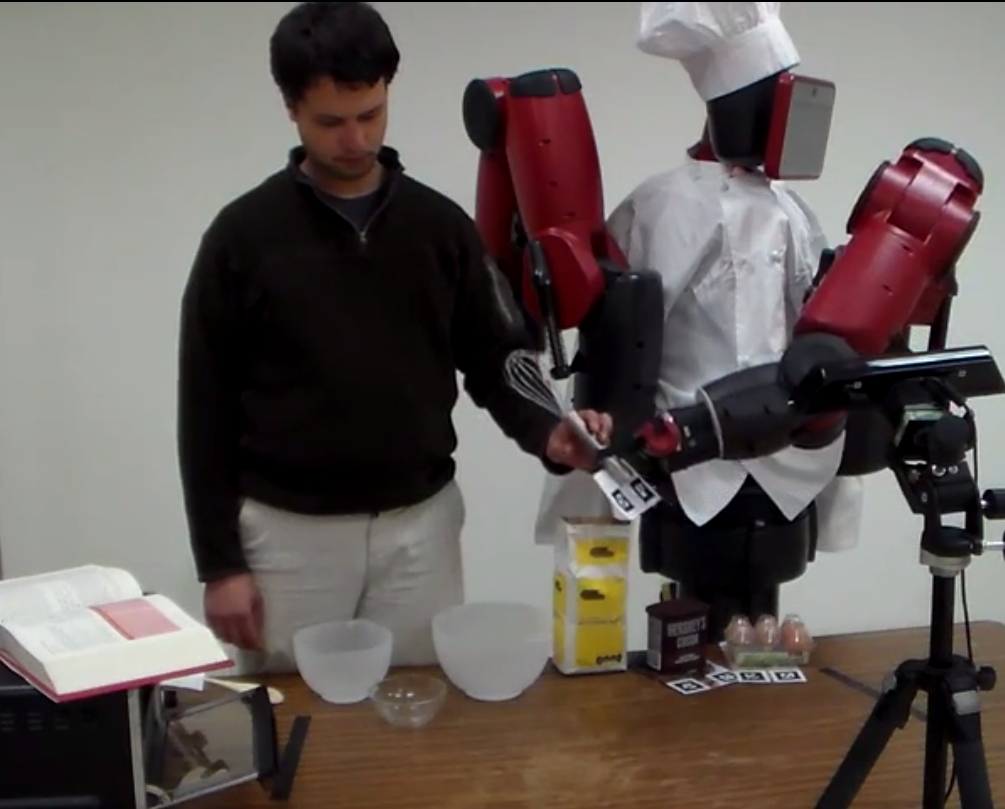
\includegraphics[width=0.75\linewidth]{figures/baxter.png}%
  \caption{Affordances enable a robot to efficiently infer helpful actions in
    very large state spaces, such as a kitchen.}
  \label{fig:baxter_results}
\end{figure}

To address this state-action space explosion, prior work has explored
adding knowledge to the planner, such as options~\cite{sutton99} and
macro-actions~\cite{Botea:2005kx,Newton:2005vn}.  However, while these
methods can allow the agent to search more deeply in the state space, they
add non-primitive actions to the planner which {\em increase} the size of
the state-action space.  The resulting augmented space is even larger,
which can have the paradoxical effect of increasing the search time
for a good policy~\cite{Jong:2008zr}.  
Deterministic forward-search algorithms like hierarchical task
networks (HTNs)~\citep{Nau:1999:SSH:1624312.1624357}, and temporal
logical planning (TLPlan)~\citep{Bacchus95usingtemporal,Bacchus99usingtemporal},
add knowledge to the planner that greatly increases planning speed, but do
not generalize to stochastic domains. Additionally, the knowledge
provided to the planner by these methods is quite extensive, reducing the
agent's autonomy.

To address these issues, we augment an Object Oriented Markov Decision Process (OO-MDP) with a formalization of {\em
  affordances}. Affordances were originally proposed by \citet{gibson77} as
action possibilities prescribed by an agent's capabilities in an environment.
%Affordances focus an agent's attention on aspects of the environment that
%are most relevant to solving its current goal and avoid exploration of irrelevant parts of the
%world.
We rigorously formalize the notion of an affordance as knowledge added
to an OO-MDP that prunes irrelevant actions on a state-by-state basis based on the agent's current goal.
Affordances can be specified by hand and also learned through
experience, making them a concise, transferable, and learnable means
of representing useful planning knowledge. Our experiments demonstrate
that affordances provide dramatic improvements for a variety of
planning tasks compared to baselines, and are applicable across
different state spaces.  Moreover, while manually provided affordances
outperform baselines, affordances learned through experience yield
even greater improvements.  We conduct experiments in the game
Minecraft, which has a very large state-action space, and on a
real-world robotic cooking assistant.  All associated code with this
paper may be found at (redacted for review).

%% Because affordances define the {\em kind} of goals for which actions
%% are useful, affordances also enable high-level reasoning that can be
%% combined with approaches like subgoal planning for even
%% greater performance gains. 

% ====== Section: Related Work ======
\section{Related Work}
\label{sec:related-work}

In this section, we discuss the differences between affordance-aware
planning and other forms of knowledge engineering that have been used
to accelerate planning.  This paper builds on previous work\footnote{A previous version
of the proposed approach may be seen planning in Minecraft at https://vimeo.com/88689171} published
at two workshops (redacted for review).

% -- Subsection: Stochastic --
\subsection{Stochastic Approaches}

Here, we compare other approaches of action pruning and
knowledge engineering that provide speedups to planners
in stochastic domains.

% --- Subsection: Temporally Extended Actions ---

Temporally extended actions are actions that the agent can select like
any other action of the domain, except executing them results in
multiple primitive actions being executed in succession. Two common
forms of temporally extended actions are {\em
  macro-actions}~\cite{hauskrecht98} ~and {\em
  options}~\cite{sutton99}.  Macro-actions are actions that always
execute the same sequence of primitive actions. Options are defined
with high-level policies that accomplish specific sub tasks. For
instance, when an agent is near a door, the agent can engage the
`door-opening-option-policy', which switches from the standard
high-level planner to running a policy that is crafted to open
doors.  Although the classic options framework is not generalizable to
different state spaces, creating {\em portable} options is a topic of
active
research~\cite{konidaris07,konidaris2009efficient,Ravindran03analgebraic,croonenborghs2008learning,andre2002state,konidaris2012transfer}.

Since temporally extended actions may negatively impact planning
time~\cite{Jong:2008zr} by adding to the number of actions the agent
can choose from in a given state, combining affordances with
temporally extended actions allows for even further speedups in
planning, as demonstrated in Table~\ref{table:temp_ext_act_results}. In
other words, affordances are complementary knowledge to options and
macro-actions.

% --- Action Pruning ---
Sherstov and Stone~\cite{sherstov2005improving} considered MDPs for
which the action set of the optimal policy of a source task could be
transferred to a new, but similar, target task to reduce the learning
time required to find the optimal policy in the target task.
Affordances prune away actions on a state-by-state basis, enabling
more aggressive pruning whereas the learned action pruning is on per-task
level.

Rosman and Ramamoorthy~\cite{rosman2012good} provide a method for
learning action priors over a set of related tasks. Specifically, they
compute a Dirichlet distribution over actions by extracting the
frequency that each action was optimal in each state for each
previously solved task.  Action priors can only be used with
planning/learning algorithms that work well with an $\epsilon$-greedy
rollout policy, while affordances can be applied to almost any MDP
solver.  Action priors are only active for a fraction $\epsilon$ of
the time steps, which is quite small, limiting the improvement they
can make to the planning speed.  Finally, as variance in tasks
explored increases, the priors will become more uniform. In contrast,
affordance-aware planning can handle a wide variety of tasks in a
single knowledge base, as demonstrated by
Table~\ref{table:minecraft_results}.

% --- Heuristics ---

Heuristics in MDPs are used to convey information about the value of a
given state-action pair with respect to the task being solved and
typically take the form of either value function
initialization~\citep{Hansen:1999qf}, or reward shaping\cite{potshap}.
However, heuristics are highly dependent on the reward function and
state space of the task being solved, whereas affordances are state
space independent and may be learned easily for different reward
functions. If a heuristic can be provided, the combination of
heuristics and affordances may even more greatly accelerate planning
algorithms than either approach alone.

% -- Subsection: Deterministic knowledge engineering approaches --
\subsection{Deterministic Approaches}

There have been several attempts at engineering knowledge
to decrease planning time for deterministic planners. These are
fundamentally solving a different problem from what we are interested
in since they deal with non-stochastic problems, but there are
interesting parallels nonetheless.

% --- Hierarchical Task Networks ---

Hierarchical Task Networks (HTNs) employ \textit{task decompositions}
to aid in planning~\cite{erol1994htn}. The agent decomposes the goal
into smaller tasks which are in turn decomposed into smaller
tasks. This decomposition continues until immediately achievable
primitive tasks are derived. The current state of the task
decomposition, in turn, informs constraints which reduce the space
over which the planner searches. At a high level HTNs and affordances
both achieve action pruning by exploiting some form of supplied
knowledge.

However HTNs do not incorporate reward into their
planning. Consequently, they lack any guarantees of the quality of any
induced plan.  Additionally, the degree of supplied knowledge in HTNs
far exceeds that of affordances: HTNs require not only constraints for
sub-tasks but a hierarchical framework of arbitrary
complexity. Affordances require either simple symbolic knowledge, as
illustrated in Table ~\ref{table:afford_kb_exp}, or a set of
predicates for use as features and a means of generating candidate
state spaces.

% --- Temporal Logic ---

Bacchus and
Kabanza~\cite{Bacchus95usingtemporal,Bacchus99usingtemporal} provided
planners with domain dependent knowledge in the form of a first-order
version of linear temporal logic (LTL), which they used for control of
a forward-chaining planner. With this methodology, a \textsc{Strips}
style planner may be guided through the search space by pruning
candidate plans that falsify the given knowledge base of LTL formulas,
often achieving polynomial time planning in exponential space.  LTL
formulas are difficult to learn, placing dependence on an expert,
while we demonstrate that affordances can be automatically learned
from experience.

% ====== Affordances ======
\section{Technical Approach}
\label{sec:affordances}

We define affordances as formal knowledge added to a Markov Decision
Process (MDP).  An MDP is a five-tuple: $\langle \mathcal{S},
\mathcal{A}, \mathcal{T}, \mathcal{R}, \gamma \rangle$, where
$\mathcal{S}$ is a state space; $\mathcal{A}$ is the agent's set of
actions; $\mathcal{T}$ denotes $\mathcal{T}(s' \mid s,a)$, the
transition probability of an agent applying action $a \in \mathcal{A}$
in state $s \in \mathcal{S}$ and arriving in $s' \in \mathcal{S}$;
$\mathcal{R}(s,a,s')$ denotes the reward received by the agent for
applying action $a$ in state $s$ and transitioning to state $s'$; and
$\gamma \in [0, 1)$ is a discount factor that defines how much the
  agent prefers immediate rewards over future rewards (the agent
  prefers to maximize immediate rewards as $\gamma$ decreases).

Our representation of affordances builds on Object-Oriented MDPs
(OO-MDPs)~\citep{diuk08}.  An OO-MDP efficiently represents the state
of an MDP through the use of objects and predicates.  An OO-MDP state
is a collection of objects, $O = \{o_1, \ldots, o_o \}$.  Each object
$o_i$ belongs to a class, $c_j \in \{c_1, \ldots, c_c\}$. Every class
has a set of attributes, $Att(c) = \{c.a_1, \ldots, c.a_a \}$, each of
which has a domain, $Dom(c.a)$, of possible values. OO-MDPs enable
planners to use predicates over classes of objects. That is, the
OO-MDP definition also includes a set of predicates $\mathcal{P}$ that
operate on the state of objects to provide additional high-level
information about the MDP state.

OO-MDP predicates provide state space independence. For a given planning domain, OO-MDP objects
often appear across tasks. Since predicates operate on collections
of objects, they generalize beyond specific state spaces within the domain.
For instance, in Minecraft, a predicate checking the contents of the agent's inventory
generalizes beyond any particular Minecraft task. We capitalize on this state space
independence by using OO-MDP predicates as features for action pruning.

% -- Subsection: Modeling the Optimal Actions --
\subsection{Modeling the Optimal Actions}

Our goal is to formalize affordances in a way that enables a planning
algorithm to prune away suboptimal actions in each state. We define
the optimal action set, $\mathcal{A}^*$, for a given state $s$ and
goal $G$ as:
% -- Equation: Optimal Action Set --
\begin{equation}
\mathcal{A}^* = \left\{ a \mid Q^*_G(s,a) = V^*_G(s) \right\}, 
\label{eq:opt_act_set}
\end{equation}
where $Q^*_G(s,a)$ and $V^*_G(s)$ represent the optimal Q function and 
value function, respectively.

We aim to learn a probability distribution over the optimality of each action
for a given state ($s$), goal ($G$), and knowledge base ($K$) by which
action pruning may be informed. Thus, we want to infer a Bernouli
distribution for each action's optimality:
% -- Equation: Master Equation --
\begin{equation}
\Pr(a_i \in \mathcal{A}^* \mid s, G, K)
\label{eq:master}
\end{equation}

\noindent for $i \in \{1, \ldots, |\mathcal{A}|\}$, where $\mathcal{A}$ is the OO-MDP action space.

We formalize our knowledge base, $K$, as a set of $n$ paired
preconditions and goal types, $\{ (p_1, g_1) \ldots (p_{n}, g_{n}) \}$,
along with a parameter vector, $\theta$. We abbreviate each pair
$(p_j, g_j)$ to $\delta_j$ for simplicity. Each precondition $p \in
\mathcal{P}$ is a {\it predicate} in predicate space, $\mathcal{P}$,
defined by the OO-MDP, and $g$ is a {\it goal type}
which is a logical expression that defines a subset of goals. For example, a
predicate might be $nearTrench(agent)$ which is true when the agent is
standing near a trench. A goal type specifies the
sort of problem the agent is trying to solve. In the context of
Minecraft, a goal type might refer to the agent retrieving an object
of a certain type from the environment, reaching a particular
location, or crafting an object or structure.  Depending on the
agent's current goal, the relevance of each action changes
dramatically.

We rewrite Equation~\ref{eq:master} replacing $K$ with its constituents:
% -- Equation: replace K --
\begin{multline}
\Pr(a_i \mid s, G, K)
= \Pr(a_i \in \mathcal{A}^* \mid s, G, \delta_1 \ldots \delta_n, \theta_i)
\end{multline}
\noindent where $\theta_i$ represents the set of parameters relevant to modeling
the probability of action $a_i \in {\cal A}^*$. 

We introduce the indicator function $f$, which returns 1 if and only if $\delta_j$'s predicate is true in the provided state $s$, and $\delta_j$'s goal type is entailed by the agent's current goal, $G$:
% -- Equation: function f defn --
\begin{equation}
f(\delta, s, G) = 
\begin{cases}
1& \delta.p(s) \wedge \delta.g(G) \\
0& \text{otherwise.}
\end{cases}
\label{eq:f_func_def}
\end{equation}

Evaluating $f$ for each $\delta_j$ given the current state and goal gives rise to a set of binary features,
$\phi_j = f(\delta_j, s, G)$, which we use to reformulate our probability distribution:
% -- Equation: replace deltas with phi --
\begin{multline}
\Pr(a_i \in \mathcal{A}^*  \mid s, G, \delta_1 \ldots \delta_n, \theta_i) \\
= \Pr(a_i \in \mathcal{A}^*  \mid \phi_1, \ldots, \phi_n, \theta_i)
\label{eq:feature_rep}
\end{multline}

This distribution may be modeled in a number of ways making this
approach quite flexible. To enable efficient learning, we model our
distribution using Naive Bayes. First we factor using Bayes' rule:
% -- Equation: Bayes --
\begin{equation}
= \frac{\Pr(\phi_1, \ldots, \phi_{n}, \mid a_i \in \mathcal{A}^*, \theta_i) \Pr(a_i \in \mathcal{A}^* \mid \theta_i)}{\Pr(\phi_1, \ldots, \phi_{n} | \theta_i)}
\label{eq:bayes}
\end{equation}

Next we assume that each feature is conditionally independent of the others, given whether the action is optimal:
% -- Equation: Naive assumption and uniform prior--
\begin{equation}
= \frac{\prod_{j=1}^{n} \Pr(\phi_j \mid a_i \in \mathcal{A}^*, \theta_i) \Pr(a_i \in \mathcal{A}^* \mid \theta_i) }{\Pr(\phi_1, \ldots, \phi_{n} | \theta_i)}
\label{eq:final}
\end{equation}

Finally, we define the prior on the optimality of each action to be
the fraction of the time each action was optimal during training.

% -- Subsection: Learning the Optimal Actions--
\subsection{Learning the Optimal Actions}
Our approach to modeling the optimality of each action allows affordances to be learned through unsupervised experience.
To learn affordances, we provide a set of training worlds ($W$) for which the optimal policy, $\pi$,
may be tractably computed. Then, we compute the maximum likelihood estimate of the parameter vector $\theta_i$ for each action.

Under our Bernouli Naive Bayes model, we estimate the parameters
$\theta_{i,0} = \Pr(a_i)$ and $\theta_{i,j} = \Pr(\phi_j | a_i)$, for $j \in \{1, \ldots, n \}$, where the maximum likelihood estimates are:
\begin{align}
\theta_{i,0} &= \frac{C(a_i)}{C(a_i) + C(\bar{a_i})} \\
\theta_{i,j} &= \frac{C(\phi_j, a_i)}{C(a_i)}
\end{align}

Here, $C(a_i)$ is the number of observed occurrences where $a_i$ was optimal across all worlds $W$,
$C(\bar{a_i})$ is the number of observed occurrences where $a_i$ was not optimal,
and $C(\phi_j, a_i)$ is the number of occurrences where $\phi_j=1$ and $a_i$ was optimal.
We determined optimality using the synthesized policy for each training world, $\pi_w$. More formally:

\begin{align}
C(a_i) &= \sum_{w \in W} \sum_{s \in w} (a_i \in \pi_w(s)) \\
C(\bar{a_i}) &= \sum_{w \in W} \sum_{s \in w} (a_i \not \in \pi_w(s) ) \\
C(\phi_j, a_i) &= \sum_{w \in W} \sum_{s \in w} (a_i  \in \pi_w(s) \wedge \phi_j == 1)
\end{align}

%Todo: Make this sound better
During the learning phase, the agent learns which actions are useful under different conditions. 
For example, consider the smelting task pictured in Figure~\ref{fig:minecraft}.
During training, we observe that the \texttt{destroyBlock} action is often optimal when the agent is looking
at a block of gold and the agent was trying to smelt gold.
Likewise, when the agent is attempting to satisfy a different goal or is {\it not} looking at a block of gold, then the \texttt{destroyBlock}
action is generally not optimal (i.e. destroying grass blocks is typically irrelevant to the smelting task). 
This information informs the distribution over the optimality of the \texttt{destroyBlock} action given the set
of features, which is used at test time to prune the action set so that the agent explores destroying blocks
when trying to smelt gold and looking at gold ore, but not in other situations (unless another affordance happens to suggest it).

% -- Figure: Minecraft pic --
\begin{figure}[b]
\centering
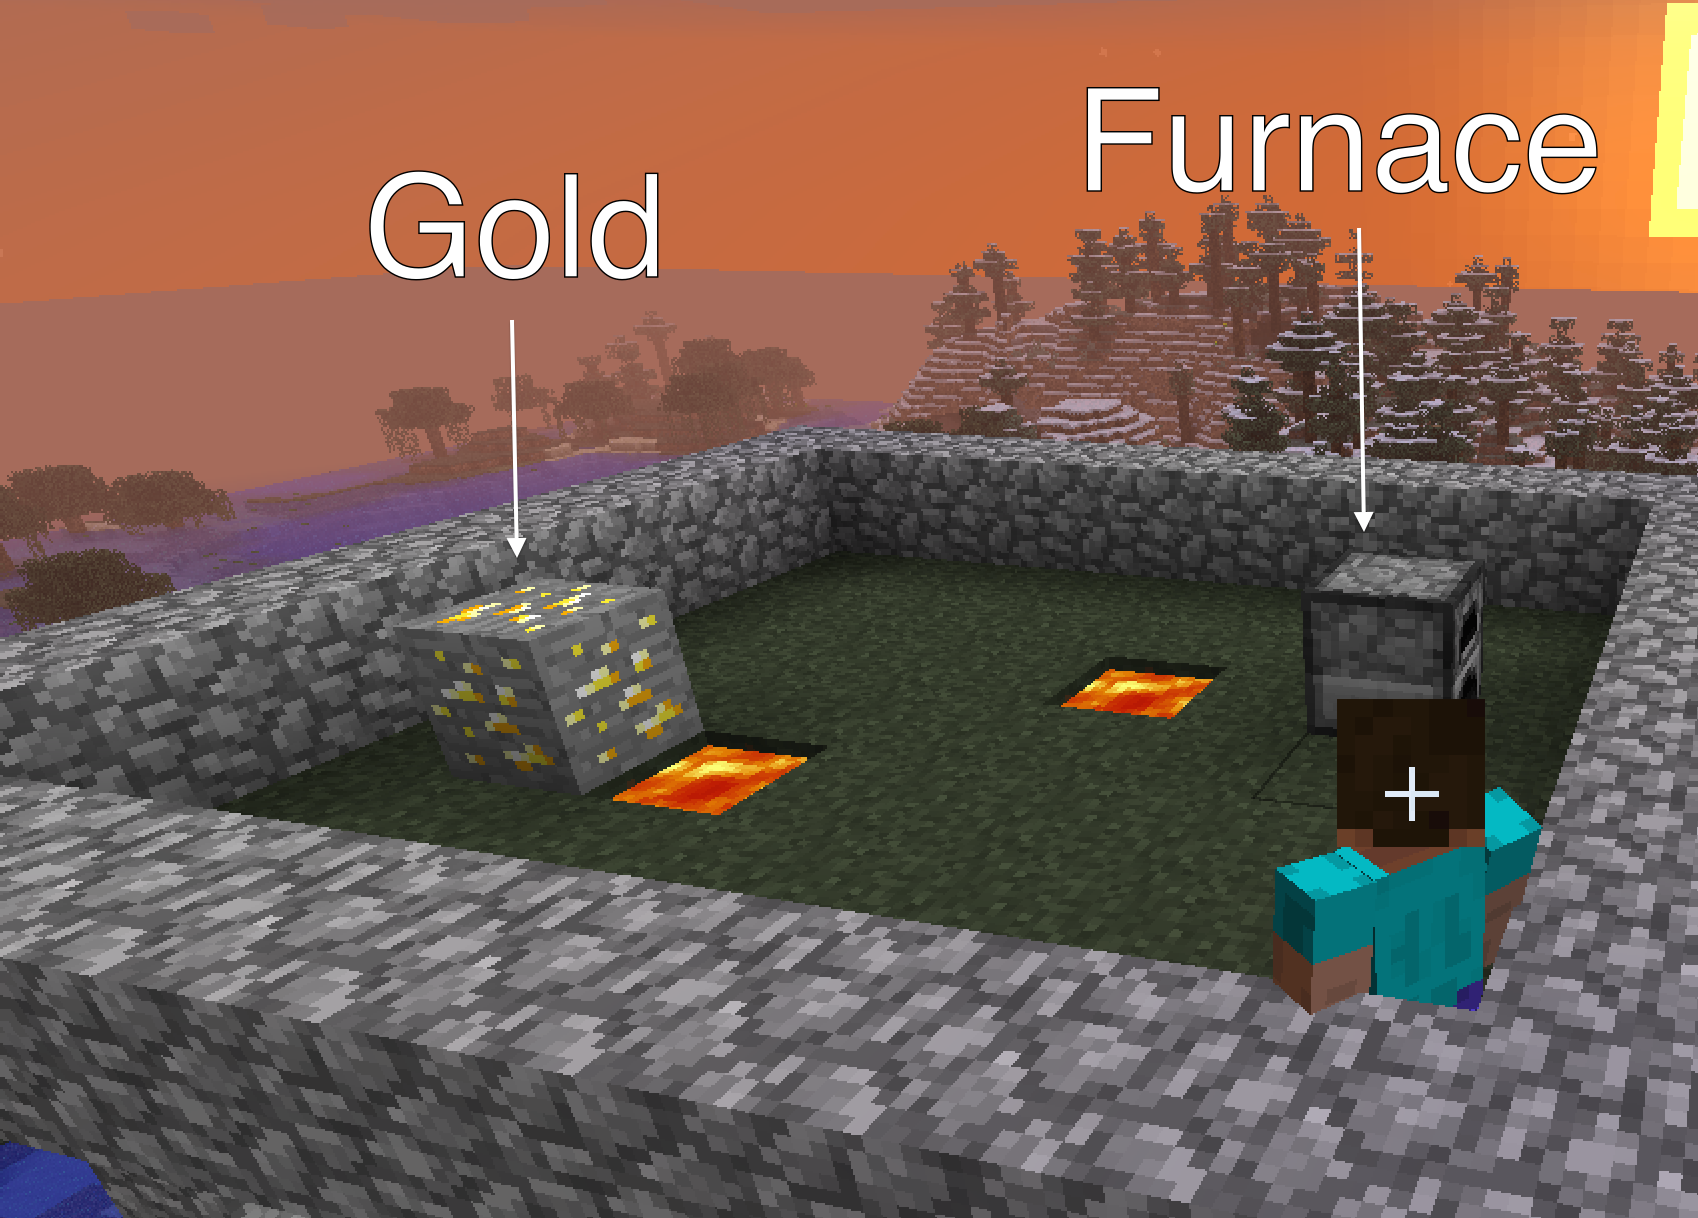
\includegraphics[scale=0.08]{figures/smelting_labeled.png}%
  \caption{A gold smelting task in the Minecraft domain.  The agent's
    goal is to mine a block of gold, move to the forge and then smelt
    the gold in the forge to produce gold ingots.}
  \label{fig:minecraft}
\end{figure}

%which actions were taken in each state. At test time, 
%when the agent is on a flat plane and needs to move to the gold ore, LRTDP will have learned
%that movement actions are useful (i.e. when the feature $\delta_j = (lookingAtGoldOre, smeltGold)$ is 0 (i.e. the agent is not looking
%at a block of gold ore or is trying to something other than smelt gold), then the probability
%that the destroy . Thus, the agent will apply the \texttt{destroyBlock}
%action when it is trying to smelt gold and is looking at gold.

% -- Subsection: Action Pruning --
\subsection{Affordance-Aware Planning}
\label{sec:action_pruning}
A planner uses affordances to prune actions in a state- and
goal-specific way.

% 1) Expert (discriminative or model)
First, affordances may be specified by a domain expert.  The expert
specifies a set of actions associated with a precondition-goal type
pair. When the affordance is active, the actions suggested by the
affordance are included in the agent's action set. For instance, if an
agent is standing above a block of buried gold and is trying to smelt
a block of gold, then an expert may indicate that the agent should
consider the actions of looking down and digging.  All actions
contributed by active affordances are grouped to yield the set of
actions to consider for each state. Table~\ref{table:afford_kb_exp}
shows several examples of expert-defined affordances.

% 2) Threshold
Second, actions may be pruned by thresholding the posterior in
Equation~\ref{eq:feature_rep}.  In this method, the affordances remove
any actions whose probability of being optimal is below the provided
threshold for each state. The threshold was determined empirically,
and was set to $\frac{0.2}{|\mathcal{A}|}$, where $|\mathcal{A}|$ is
the size of the full action space of the OO-MDP.  This threshold is
quite conservative, and means that our approach only prunes actions
which are extremely unlikely to be optimal.

% 3) Sampling
%% Lastly, actions may be pruned by sampling actions from the posterior,
%% treating each action's probability mass as a Bernouli trial and
%% sampling across the entire action set. In preliminary results, this
%% method did not perform as well as baselines - likely because the
%% weights associated with each action were too small. In future work, we
%% are interested in investigating more sophisticated approaches to
%% pruning actions with sampling.

Through the use of any of the above methods, an affordance-aware
planner prunes actions on a state-by-state basis, focusing the agent
on relevant action possibilities of the environment, consequently
reducing planning time. Any planner operating in an OO-MDP may be made
affordance-aware with this approach.


% -- Table: Expert provided affordances --
\begin{table}[t]
\ra{1.15}
\small
\begin{tabular}{@{}llll@{}}\toprule
Precondition & Goal Type & Actions \\ \midrule
\texttt{lookingTowardGoal} & \texttt{atLocation} & \texttt{\{move\}} \\
\texttt{lavaInFront} & \texttt{atLocation} & \texttt{\{rotate\}} \\
\texttt{lookingAtGold} & \texttt{hasGoldOre} & \texttt{\{destroy\}} \\
\bottomrule
\end{tabular}

\caption{Examples of expert-provided affordances.\label{table:afford_kb_exp}}
\end{table}

In a recent review on the theory of affordances,~\citet{chemero2003}
suggests that an affordance is a relation between the features of an
environment and an agent's abilities. Our approach grounds this
interpretation, where the features of the environment correspond to
the goal-dependent state features, $\phi$, and the agent's abilities
correspond to the OO-MDP action set. In our model, there is an
affordance for each $\delta_j$, with preconditions $\delta_j.p$, goal
type $\delta_j.g$ and action distribution $\Pr(a_i \in \mathcal{A}^* | \phi_j,
\theta)$, which is computed in our Naive Bayes model by marginalizing
over all the features not associated with $\phi_j$.

%As with human agents, multiple affordances often inform decision
%making at a given time.  Thus, affordance-aware planning agents
%operating within an OO-MDP will rarely make specific reference to
%particular affordances, but will instead reason about the world using
%the relevant action possibilities identified by the distribution in
%Equation~\ref{eq:final}.  That said, individual affordances can still
%be specified by experts, providing a natural spectrum between
%expert-provided knowledge and learned knowledge.

% ====== Section: Results ======
\section{Results}
\label{sec:results}

% Move average results HERE if want to go back to old method

We evaluate our approach using the game Minecraft and a collaborative
robotic cooking task.  Minecraft is a 3-D blocks game in which the
user can place, craft, and destroy blocks of different types.
Minecraft's physics and action space allow users to create complex
systems, including logic gates and functional scientific graphing
calculators\footnote{https://www.youtube.com/watch?v=wgJfVRhotlQ}.
Minecraft serves as a model for robotic tasks such as cooking
assistance, assembling items in a factory, object retrieval, and
complex terrain traversal.  As in these tasks, the agent operates in a
very large state-action space in an uncertain environment.
Figure~\ref{fig:minecraft} shows a scene from one of our Minecraft
problems.  Additionally, we implemented an affordance based planner to
enable a manipulator robot to infer helpful actions in response to a
person working on a kitchen task, shown in Figure~\ref{fig:baxter_results}.

% -- Subsection: Minecraft Tests --
\subsection{Minecraft Tests}

Our experiments consisted of five common tasks in Minecraft, including
constructing bridges over trenches, smelting gold, tunneling through
walls, basic path planning, and digging to find an object.  We tested
on randomized worlds of varying size and difficulty. The generated
test worlds varied in size from tens of thousands of states to
hundreds of thousands of states.  The agent learned affordances from a
training set consisting of 20 simple state spaces of each map type
(100 total maps), each approximately a 1,000-10,000 state world. We
conducted all tests with a single knowledge base.

We use Real Time Dynamic Programming (RTDP)~\cite{barto95} as our
baseline planner, a sampling-based algorithm that does not require the
planner to visit all states. We compare RTDP with learned
affordance-aware RTDP (LRTDP), and expert-defined affordance-aware
RTDP (ERTDP). We terminated each planner when the maximum change in
the value function was less than 0.01 for 100 consecutive policy
rollouts, or the planner failed to converge after 1000 rollouts.  The
reward function was $-1$ for all transitions, except transitions to
states in which the agent was in lava, where we set the reward to
$-10$. The goal was set to be terminal. The discount factor was
$\lambda = 0.99$.  To introduce nondeterminism into our problem,
movement actions (move, rotate, jump) in all experiments had a small
probability (0.05) of incorrectly applying a different movement
action.  This noise factor approximates noise faced by a physical
robot that attempts to execute actions in a real-world domain.

% -- Figure: Average results --
\begin{figure}[t]
%\begin{figure}
\centering
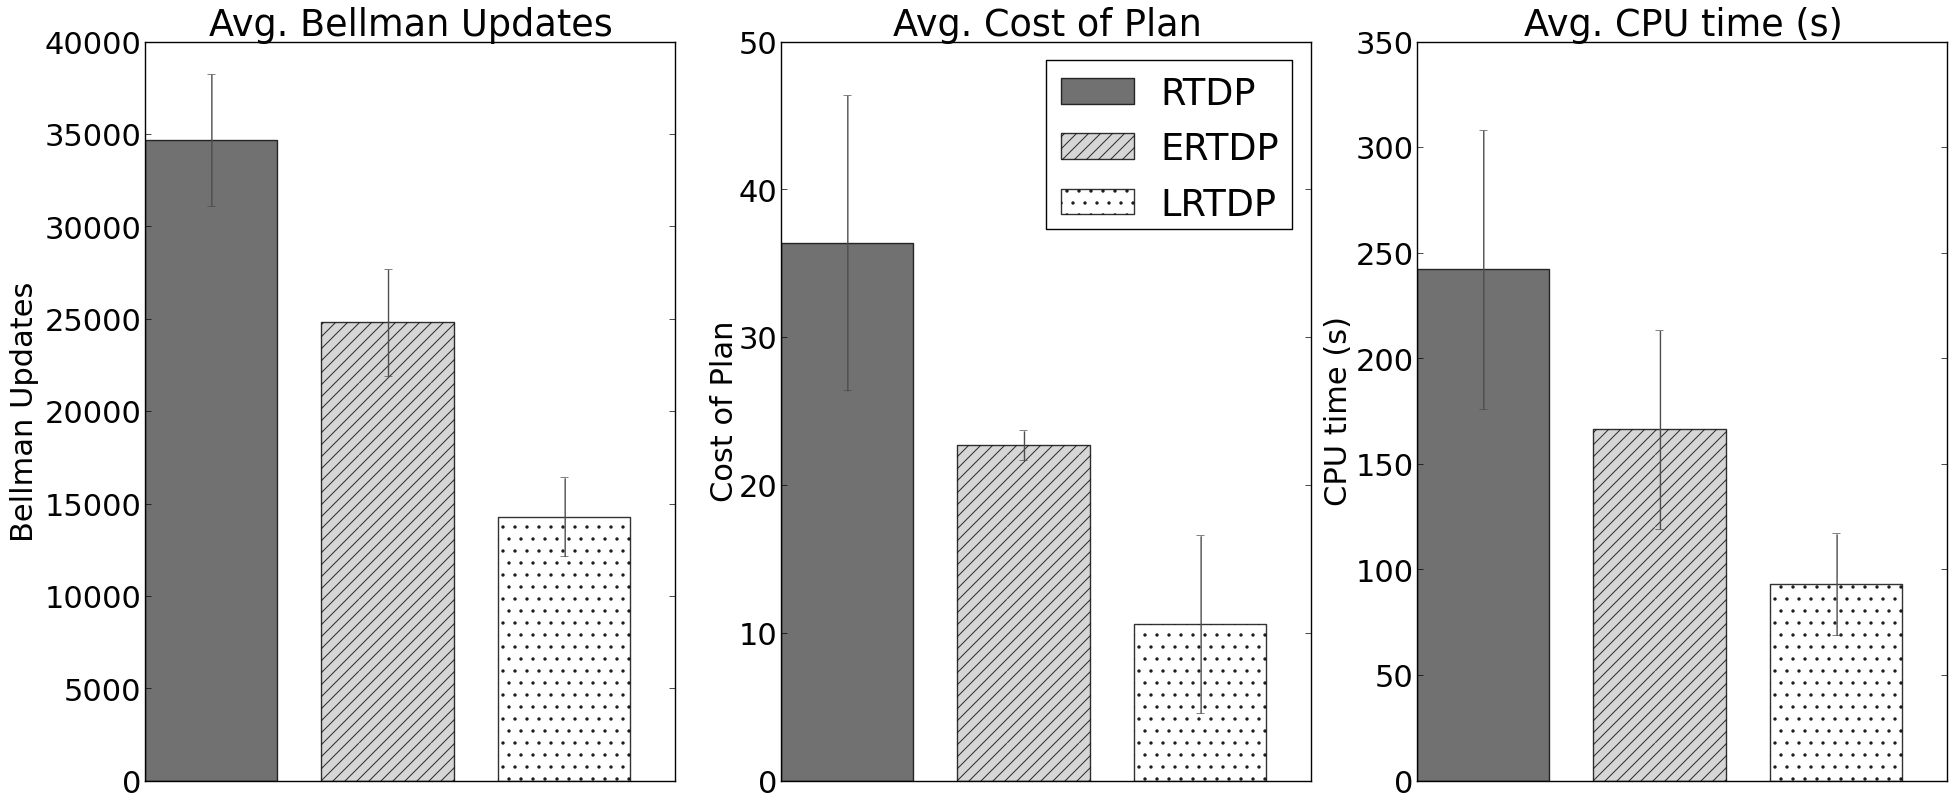
\includegraphics[width=1\linewidth]{figures/average_results_cropped.png}%
%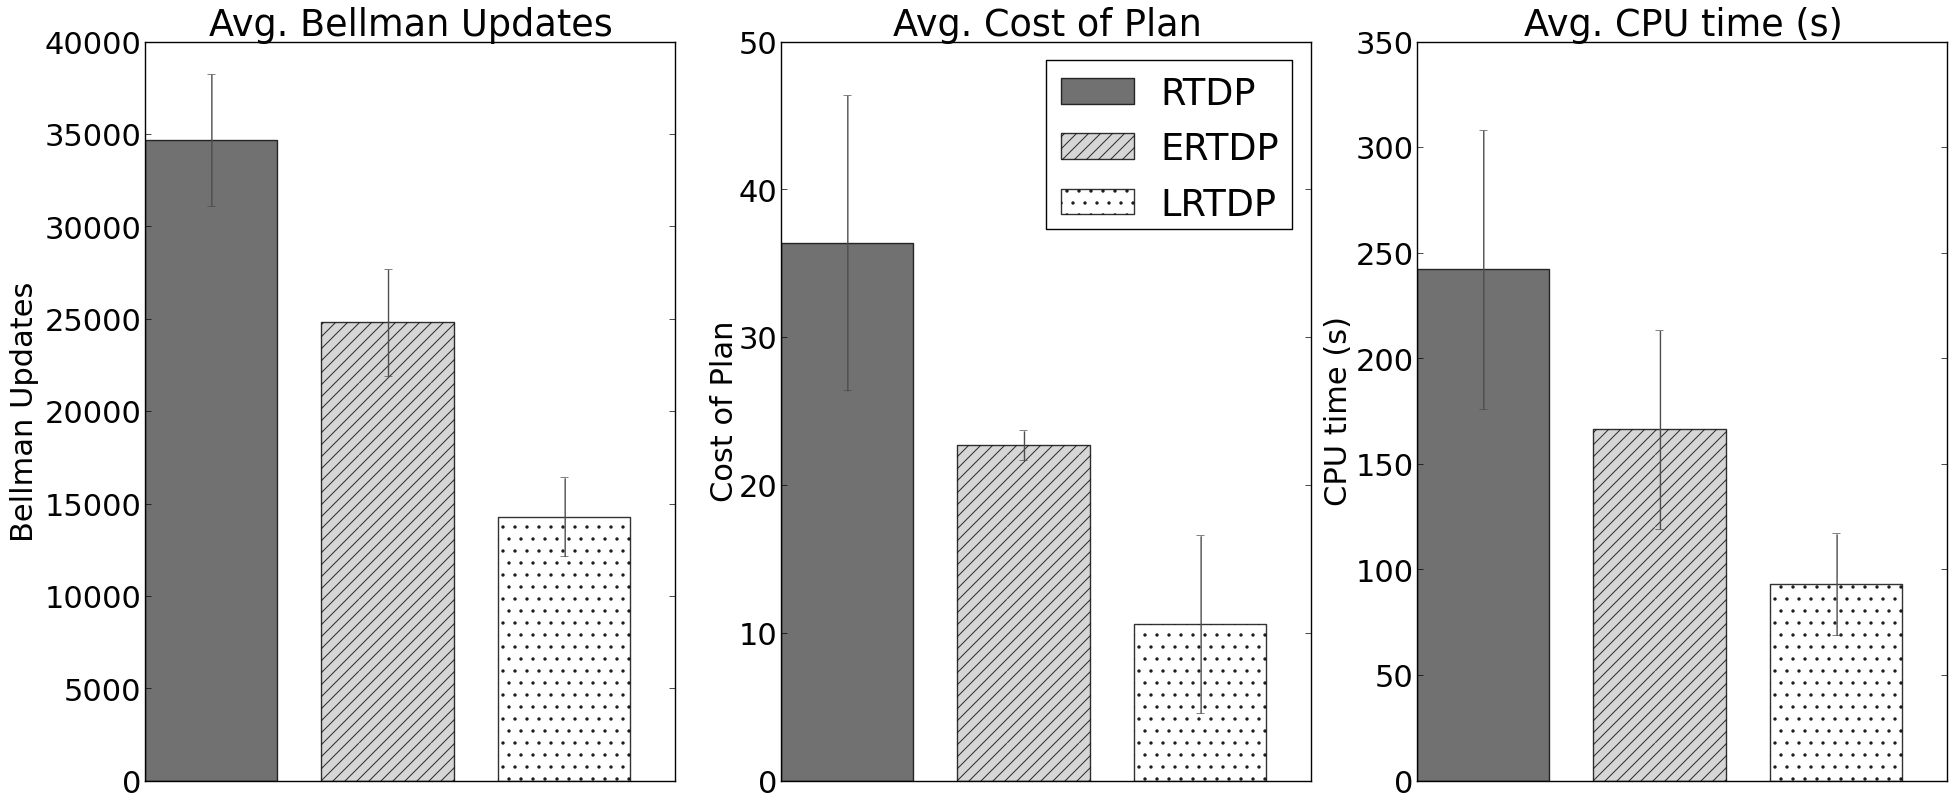
\includegraphics[scale=0.18]{figures/average_results_cropped.png}%
\caption{Average results from all maps.}
\label{fig:average_results}
\end{figure}
%\end{figure}

We report the number of Bellman updates executed by each planning
algorithm, the accumulated reward of the average plan, and the CPU
time taken to find a plan. Table~\ref{table:minecraft_results} shows
the average Bellman updates, accumulated reward, and CPU time for
RTDP, LRTDP and ERTDP after planning in 20 different maps of each goal
type (100 total). Figure~\ref{fig:average_results} shows the results
averaged across all maps.

% -- Table: Minecraft results --
\begin{table}[t]
\ra{1.15}
\small
\begin{tabular}{@{}llll@{}}\toprule
Planner & Bellman & Reward & CPU \\ \midrule
&\hspace{-10mm}{\it Mining Task} \\
\texttt{RTDP} & 17142.1 ($\pm$3843) 		& {\bf -6.5} ($\pm$1)  & {\bf 17.6s}   ($\pm$4) \\
\texttt{ERTDP} 	& 14357.4 ($\pm$3275) 		& {\bf -6.5}   ($\pm$1) & 31.9s   ($\pm$8) \\
\texttt{LRTDP} 	& {\bf 12664.0} ($\pm$9340) 	& -12.7 ($\pm$5) & 33.1s   ($\pm$23) \\\hline
&\hspace{-10mm}{\it Smelting Task} \\
\texttt{RTDP} 	& 30995.0 ($\pm$6730) 		& {\bf -8.6}   ($\pm$1) & 45.1s   ($\pm$14) \\
\texttt{ERTDP} 	& 28544.0 ($\pm$5909) 		& {\bf -8.6}   ($\pm$1) & 72.6s   ($\pm$19) \\ 
\texttt{LRTDP} 	& {\bf 2821.9} 	 ($\pm$662) 	& -9.8   ($\pm$2) & {\bf 7.5s}  ($\pm$2) \\ \hline
&\hspace{-10mm}{\it Wall Traversal Task} \\
\texttt{RTDP} & 45041.7 ($\pm$11816) 		& -56.0   ($\pm$51) & {\bf 68.7s}   ($\pm$22) \\
\texttt{ERTDP} 	& 32552.0 ($\pm$10794) 		& -34.5   ($\pm$25) & 96.5s   ($\pm$39) \\ 
\texttt{LRTDP} 	& {\bf 24020.8} ($\pm$9239) 	& {\bf -15.8}   ($\pm$5) & 80.5s   ($\pm$34) \\ \hline
&\hspace{-10mm}{\it Trench Traversal Task} \\
\texttt{RTDP}  	& 16183.5 ($\pm$4509) 		& {\bf -8.1}   ($\pm$2) & 53.1s   ($\pm$22) \\
\texttt{ERTDP} 	& {\bf 8674.8} 	($\pm$2700) 	& -8.2   ($\pm$2) & {\bf 35.9s}   ($\pm$15) \\ 
\texttt{LRTDP} 	& 11758.4 ($\pm$2815) 		& -8.7   ($\pm$1) & 57.9s   ($\pm$20) \\ \hline
&\hspace{-10mm}{\it Plane Traversal Task} \\
\texttt{RTDP} & 52407 ($\pm$18432) 		& -82.6   ($\pm$42) & 877.0s   ($\pm$381) \\
\texttt{ERTDP} 	& 32928 ($\pm$14997) 		& -44.9   ($\pm$34) & 505.3s   ($\pm$304) \\
\texttt{LRTDP} 	& {\bf 19090} 	 ($\pm$9158) 	& {\bf-7.8}   ($\pm$1) & {\bf 246s}  ($\pm$159) \\
\bottomrule
\end{tabular}
\caption{RTDP vs. affordance-aware alternatives.}
\label{table:minecraft_results}
\end{table}

Because the planners were forced to terminate after only 1000
rollouts, they did not always converge to the optimal policy. LRTDP on
average found a comparably better plan (10.6 cost) than ERTDP (22.7
cost) and RTDP (36.4 cost), found the plan in significantly fewer
Bellman updates (14287.5 to ERTDP's 24804.1 and RTDP's 34694.3) and in
less CPU time (93.1s to ERTDP's 166.4s and RTDP's 242.0s).  These
results indicate that while learned affordances gave the largest
improvements, expert-provided affordances can also significantly
enhance performance, and, depending on the domain, could add
significant value in making large state-spaces tractable without the
overhead of supplying training worlds.

%Todo: Make this paragraph better
For some task types, LRTDP found a slightly worse plan on average than
vanilla RTDP (e.g. the mining task). This is due to the fact that LRTDP
occasionally prunes actions that are essential for solving a particular problem (such as
pruning the \texttt{destroyBlock} action in certain states of the mining task).
To fix this, we could lower the threshold to allow for even more conservative action pruning
at the cost of additional computation. In future work, we plan on investigating approaches
to dynamically adjusting the threshold based on planning feedback.

%\stnote{We need to explain the results in Table 3 about why
%  affordances don't always help.  Why is the reward sometimes worse
%  with affordances?  Why is the runtime sometimes worse? W hat is
%  special about the domains where that is happening?}


\begin{table}[b]
\ra{1.15}
\small
\begin{tabular}{@{}llll@{}}\toprule
Planner & Bellman & Reward & CPU \\ \midrule
\texttt{RTDP}   			&	27439 ($\pm$2348)		&	-22.6 ($\pm$9)		& 107 ($\pm$33) \\
\texttt{LRTDP} 			& 	{\bf 9935} ($\pm$1031)	&	{\bf -12.4} ($\pm$1)& {\bf 53} ($\pm$5) \\ \hline
\texttt{RTDP+Opt}  		&	26663 ($\pm$2298)		&	-17.4 ($\pm$4) 		& 129($\pm$35) \\
\texttt{LRTDP+Opt} 		& 	{\bf 9675} ($\pm$953)	&	{\bf -11.5} ($\pm$1)	&{\bf 93} ($\pm$10) \\ \hline
\texttt{RTDP+MA}  		&	31083 ($\pm$2468)		&	-21.7	 ($\pm$5)		&336 ($\pm$28) \\
\texttt{LRTDP+MA}  		& 	{\bf 9854} ($\pm$1034)	&	{\bf -11.7} ($\pm$1)	&{\bf 162} ($\pm$17) \\ %\hline
%\texttt{RTDP+MA+Opt}  	&	27143($\pm$2380)		&	-16.9($\pm$3.0)	&	323($\pm$38)		\\ 
%\texttt{LRTDP+MA+Opt} & 	{\bf 10622($\pm$1046)}	&	{\bf -13.4($\pm$1.0)}	&	{\bf 237($\pm$29)}		\\
\bottomrule
\end{tabular}
\caption{Affordances vs. Temporally Extended Actions}
\label{table:temp_ext_act_results}
\end{table}


% -- Subsection: Temporally Extended Actions --
\subsection{Temporally Extended Actions and Affordances}

We compared our approach to Temporally Extended Actions: macro-actions
and options. We conducted these experiments with the same
configurations as our Minecraft experiments. Domain experts provided
the option policies and macro-actions.

Table~\ref{table:temp_ext_act_results} indicates the results of
comparing RTDP equipped with macro actions, options, and affordances
across 100 different executions in the same randomly generated
Minecraft worlds. The results are averaged across tasks of each type
presented in Table~\ref{table:minecraft_results}. Both macro-actions
and options add a significant amount of time to planning.  This
increase is because it is computationally expensive to predict the
expected reward associated with applying an option or a
macro-action. Furthermore, the branching factor of the state-action
space significantly increases when augmented with additional actions,
causing the planner to run for longer and perform more Bellman
updates. With affordances, the planner found a better plan in less CPU
time, and with fewer Bellman updates. These results support the claim
that affordances can handle the augmented action space provided by
temporally extended actions by pruning away unnecessary actions, and
that options and affordances provide complementary information.

% -- Subsection: Baxter --
\subsection{ERTDP and Baxter}

To assess affordances applied to a real-world robotic task, we devised
a cooking domain that requires the robot to choose helpful actions for
a person following a recipe.  The robot reasons over ingredients,
containers, appliances, working spaces and utensils. The action set
consists of pouring containers, mixing ingredients and moving containers and tools, 
encapsulating a large set of grounded actions for
the objects in a kitchen.

% -- Figure: Baxter results/image

To help a person cook, a robot needs to plan across possible actions a
person might take as well as possible actions the robot could take.
Coupled with the large number of items in a kitchen, a planner in this
complicated world must take advantage of knowledge inherent to the
domain and to the recipe with which it is working. Using four ingredients 
required for brownies and the containers necessary for the ingredients, our
cooking state space has $\num[round-precision=3, round-mode=figures]{47258883}$ states.  
%To remove a large number of self-transitions, we provided affordances for each
%action. For example, one affordance specified that mixing should only occur 
%in containers that contain ingredients. An affordance for pouring required 
%the container being poured to contain ingredients. 

We divided a brownie recipe into three subgoals: combining and mixing the dry ingredients,
combining and mixing the wet ingredients, and combining these two
mixtures into a batter. For each subgoal, we provided more
affordances specific to the objects used in that subgoal, like a whisk should
only be used to mix wet ingredients.  
We used ERTDP to search for the least-cost plan
to complete the recipe.  The robot inferred actions such as handing
off the whisk to the person to mix the wet ingredients.

\begin{table}[t]
\ra{1.1}
\small
\begin{tabular}{@{}llll@{}}\toprule
Planner & Bellman & Reward & CPU \\ \midrule
&\hspace{-10mm}{\it Dry Ingredients} \\
\texttt{RTDP} 	& 20000 ($\pm$0) 			& {-123.1} ($\pm$0)  & {56.0s}   ($\pm$2.9) \\
\texttt{ERTDP} 	& {\bf 2457.2} ($\pm$53.2) 		& {\bf -6.5}   ($\pm$0) & {\bf 10.1s}   ($\pm$0.3) \\  \hline
&\hspace{-10mm}{\it Wet Ingredients} \\
\texttt{RTDP} 	& 19964 ($\pm$14.1) 			& { -123.0}   ($\pm$0) & 66.6s   ($\pm$9.9) \\
\texttt{ERTDP} 	& {\bf 5873.5} ($\pm$53.7) 		& {\bf -6.5}   ($\pm$0) & {\bf 15.6s}   ($\pm$1.2) \\ \hline
&\hspace{-10mm}{\it Brownie Batter} \\
\texttt{RTDP} 	& 20000 ($\pm$0) 			& -123.4   ($\pm$0.7) & { 53.3s}   ($\pm$2.4) \\
\texttt{ERTDP} 	& {\bf 6642.4} ($\pm$36.4) 		& {\bf -7.0}   ($\pm$0) & {\bf 31.9s}   ($\pm$0.4) \\ 
\bottomrule
\end{tabular}
\caption{RTDP vs. ERTDP for robotic kitchen tasks}
\label{table:baxter_results}
\end{table}

In table~\ref{table:baxter_results} we show the comparison between
standard RTDP and ERTDP for the three subgoals. Because the
state-action space is reduced significantly,
ERTDP can plan successfully in a short amount of time. Standard RTDP always encountered
the maximum number of rollouts specified at the maximum depth each time.

We provide a video\footnote{Watch at https://vimeo.com/106226282} 
showing how this affordance-aware planner running
on a robot can help a person cook by dynamically replanning through
constant observations. After observing the placement of a cocoa
container in the robot's workspace, the robot fetches a wooden spoon
to allow the person to mix. After observing an egg container, the
robot fetches a whisk to help beat the eggs. Because we modeled the
culinary world as an MDP and replanned at every observation, the robot
dynamically resolves failures and accounts for unpredictable user
actions. In the video, the robot fails to grasp the wooden spoon on
the first attempt and must retry the grasp after it observed no state
change.

% ====== Section: Conclusion ======
\section{Conclusion}
\label{sec:conclusion}
We proposed a novel approach to represent transferable planning
knowledge in terms of {\em affordances}~\cite{gibson77}. Affordances
allow an agent to efficiently prune actions based on learned or expert
provided knowledge, significantly reducing the number of state-action
pairs the agent needs to evaluate in order to act near optimally. We
demonstrated the effectiveness of the affordance model by comparing
RTDP to its affordance-aware equivalents in a series of challenging
planning tasks in the Minecraft domain. Further, we designed a
learning process that allows an agent to autonomously learn useful
affordances that may be used across a variety of task types, reward
functions, and state spaces, allowing for convenient extensions to
robotic applications.  Additionally, we compared the effectiveness of
augmenting planners with affordances with temporally extended actions,
and the combination of the two. The results suggest that affordances
may be combined with temporally extended actions to provide
improvements in planning.  Lastly, we deployed an affordance-aware
planner on a robot in a collaborative cooking task.

In the future, we hope to automatically discover useful state space
specific subgoals online - a topic of some active research
\cite{Mcgovern01automaticdiscovery,Simsek:2005:IUS:1102351.1102454}.
Automatic discovery of subgoals would allow affordance-aware planners
to take advantage of the goal-oriented focus of affordances, and would
further reduce the size of the explored state-action space by
improving the effectiveness of action pruning.

Additionally, we hope to explore additional methods that capitalize on
the distribution over optimal actions, such as incorporating
affordances with a forward search sparse sampling
algorithm~\cite{walsh2010integrating}, or replacing the Naive Bayes
model with a more sophisticated model, such as Logistic Regression or
a Noisy-OR.  We are also investigating methods of learning the
threshold value in a more principled way - one such approach is to
initialize the planner with a strict threshold, and slowly relax the
threshold until a near optimal policy is found.  These methods will
enable agents to acquire and leverage general planning knowledge to
infer actions in very large state spaces.

{\small
\bibliographystyle{plainnat}
\bibliography{main}
}
\end{document}


